%%%%%%%%%%%%%%%%%%%%% chapter.tex %%%%%%%%%%%%%%%%%%%%%%%%%%%%%%%%%
%
% sample chapter
%
% Use this file as a template for your own input.
%
%%%%%%%%%%%%%%%%%%%%%%%% Springer-Verlag %%%%%%%%%%%%%%%%%%%%%%%%%%
%\motto{Use the template \emph{chapter.tex} to style the various elements of your chapter content.}
\chapter{智能客服系统}
\label{basic} % Always give a unique label
% use \chaptermark{}
% to alter or adjust the chapter heading in the running head


\section{简介}
现在越来越多的交易和交流都可以通过网上平台完成,如果顾客在使用产品中碰到问题,他们可以在随时在网上提问,跟客服交流。传统公司会雇佣客服专员来回应客服的问题,然而提问高峰期的时候因为人太多,顾客不得不等待很长时间;深夜凌晨的时候客服下班,顾客的问题得不到解答。如果传统公司雇佣一大批客服专员24小时值班,那导致的人工成本会非常高昂。智能客服系统使用人工智能技术进行问题语义分析,答案查找,可以自动完成问答,能提高顾客的用户体验,大大降低公司所需客服专员数量。智能客服系统的速度很快,可以同时回答很多顾客的问题,而且可以7*24小时在线不会下班,价格也比人工客服更经济实惠。

\section{问题形式化定义}
此处客服系统假设客人和客服专员通过文字进行交流。智能客服系统会根据用户输入的问题和当前聊天语境,输出对应的文字解答。我们用$\bf{X}$来代表用户的输入,用$\bf{Y}$来代表系统的输出。客服系统可以表示为
$$\bf{Y} = f(\bf{X}).$$

根据客服系统的功能不同,一般分为检索型对话系统,任务型对话系统\cite{young2013pomdp}和生成型对话系统\cite{sutskever2014sequence,shang2015neural,serban2016building,serban2016hierarchical}。
% 介绍不同对话系统的结合方法
工业应用中,一个完整的对话系统可能会同时包含以上三种对话系统。
% TODO:需要补充一个流程图
对于一个用户的提问,任务型对话系统首先要判断用户是否要开始一个任务,如果是任务则交由任务式对话系统负责;然后检索性对话系统判断用户是否在询问某个知识点,如果是则回复对应的知识点;如果不是以上两种意图,则使用生成式对话系统来进行闲聊回复。

\section{检索型对话系统}
% 定义
顾名思义,检索式模型就是查找问题库中跟当前问题最相似的问答对,输出答案。
% 好处
检索型对话系统适用于能一句话就能描述清楚的问题,而且答案比较固定不会经常变动的情况。这样的例子包括``你们公司的地址是哪里?''和``你们的咨询电话是多少?''这类简单问题。

检索模型可以形式化地表现为
$$\bf{Y} = \text{argmax}_{\bf{Y}} s(\bf{X},\bf{X}_i), \forall <\bf{X}_i,\bf{Y}_i> \in \mathcal{D}$$.
% 模块包括
检索式对话系统一般包括问题库$\mathcal{D}$,问题匹配模型$s(\bf{X}_1,\bf{X}_2)$两个部分。问题库记录了常见问题和标准的回答,而匹配模型会计算用户的输入问句$\bf{X}$跟问题库中的所有问题$\mathcal{D}=\{<\bf{X}_i,\bf{Y}_i>\}_{i=0}$之间的匹配度,系统输出最高的问题的标准答案。

% 核心问题
检索式对话系统的核心在于问题匹配模型,就是如何计算用户输入问题跟标准问题库之间的相似度。

读者可能很容易就可以想到的一种方法就是对所有的输入问题,经过分词,提取TF-IDF特征,然后使用两个问题的特征向量来计算问题之间的相似度。
% 好处,简单直观,不需要训练数据
% 困难
由于自然语言中,问题本身的表述形式非常多样,难以穷尽。这种人工特征的性能有很大改进空间,经常对同一种意思的几种不同说法不是太鲁棒。

基于深度学习的句子语义匹配,可以在训练集模型上学习把意思相近,可是说法不一样的一对句子映射到相似的语义空间中去。常见的深度学习匹配模型包括基于语义表示的匹配模型,基于交互的语义表示模型。经过训练之后的深度语义匹配模型可以把测试集中相同意思可是不同说法的两个句子也表示成相似,增加了方法的泛化能力。
% 困难
基于深度学习的句子匹配模型复杂,一般来说需要大量的训练数据才能训练好。有一些工作为了减少所需要的训练数据,他们提出了利用大数据上预训练的NLP模型来对深度语义模型进行初始化,取得了良好的效果。

检索性对话系统的缺点包括问题库更新困难,标准答案不能实时变动等。

\section{多轮任务型对话系统}
% 定义
多轮任务型对话系统\cite{young2013pomdp},又称填槽型对话系统,会通过提问,来引导用户提供完成当前任务所需的多个关键信息``槽位'',进而帮用户完成复杂任务。
% 好处
多轮任务型对话系统适用于不能用一句话描述清楚的,需要多轮交流才能完成的问题,这样的例子包括购买机票,预定酒店等。

% 模块包括
第$n$个用户输入可以表示为$\bf{X}_n$, 第$n$个系统回复可以表示为$\bf{Y}_n$,第n轮对话的对话记录可以标记为$\bf{H}_n=\{ \{\bf{X}_i,\bf{Y}_i\}_{i=1}^{n-1}, \bf{X}_n\}$。多轮对话系统可以被形式化地表示为
$$\bf{Y}_n = f(\bf{H}_n).$$
多轮任务型对话系统跟单轮系统不一样的是,任务型系统需要考虑对话的状态。对于一个任务,设计者需要指定完成要获取哪些槽位信息$\{s_i\}$,而在对话过程中,每一个信息的获取情况,就可以认为是对话的状态。例如在定机票任务中,需要获取的槽位包括``起飞时间'',``起飞城市'',``到达城市''等,而对话状态$\tilde{\bf{H}}_n$就是这些槽位的获取状态,假设每个槽位都只有获取完成和未获取两种状态,那订机票任务的对话状态一共有$2^3=8$个。

% 核心问题
多轮任务型对话系统包括四个模块,自然语言理解模块,对话状态跟踪模块,对话策略模块和自然语言生成模块。口语理解模块自然语言理解模块会根据对话的每一轮输入$\bf{X}_n$,从用户的问题中识别出用户的意图$a_n$和槽位值$\bf{s}_n=\{s_i=v_i\}$。
对话状态跟踪模块会根据当前的对话记录$\bf{H}_n$,计算最新的对话状态$\tilde{\bf{H}}_n$。 对话策略模块会根据最新的对话状态$\tilde{\bf{H}}_n$计算系统的回复动作$a'_n$和回复槽位值$\bf{s}'_n=\{s_i=v_i\}$。自然语言生成模块会根据回复动作$a'_n$和回复槽位值$\bf{s}'_n=\{s_i=v_i\}$生成回复的句子$\bf{Y}_n$。

% 常见实现方法
这里介绍一下四个模块的常见实现方法。
其中自然语言理解模块可以分为口语预处理,语义切割,语义去噪,意图识别和词槽识别四个主要部分。用户在与智能客服系统,尤其是语音智能客服交流问题的时候,其输入带有很强的口语化特征,例如在用户问句“你好我那个那个问个问题啊我的还款逾期逾期了要咋整哦”中,口语化特征包括招呼语“你好”,重复“那个那个”和“逾期逾期”,无关短语“问个问题啊”以及口语“要咋整哦”。口语化处理部分会先处理这些招呼语,重复和一些无用的语气词“哦”。使得整个句子更加干净。

口语输入还有个问题是用户会说很长一段话或敲很长一段文字,所以在初步口语处理过后需要有一个语义切割的模块来将句子切割成小片段。实践中一般会按照句号或者逗号两种尺度来切割句子。句号分割的会有完整的转折或者因果关系,比如“我的还款逾期了要咋整”。逗号分隔的会把语言切割成比较小的粒度,比如“问个问题”,“我的还款逾期了”和“要咋整”,小的粒度比较好理解。 两种尺度结合起来实现更全面的语言理解。

接下来语义去噪部分会把“问个问题”这样与任务无关的短语识别出来,词槽识别会把“我的还款逾期了”识别成“还款状态:逾期”,意图识别会把“要咋整”识别成意图“如何操作”。意图识别部分和语义去噪部分都可以使用文本分类模型,常见的文本分类深度学习模型有TextCNN\cite{kim-2014-convolutional},RCNN\cite{lai2015recurrent}和HAN\cite{yang2016hierarchical}等。词槽识别和语义切割都可以使用序列标注模型,现在比较流行是BERT+LSTM+CRF。

\begin{figure}[H]
\centering
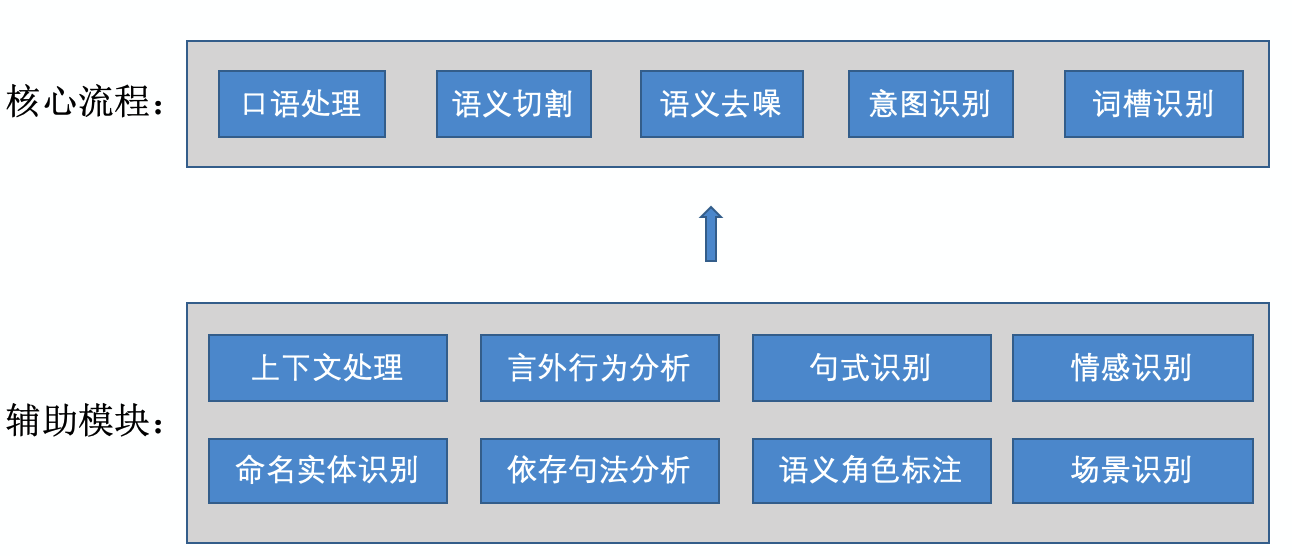
\includegraphics[scale=0.25]{chapters/nlu_process.png}
\caption{自然语言理解模块主要组成部分}
\label{fig:parserexample}
\end{figure}

自然语言理解部分还有一些比较重要的模块比如句式识别,用户言外行为识别,上下文处理模块,场景识别模块,情感识别模块,依存语法分析模块和语义角色识别模块。其中句式识别主要用来识别是陈述句还是疑问句,疑问句会被优先输入意图识别模块,陈述句会被优先输入词槽抽取模块。用户言外行为识别可以用来识别用户是否在发出请求或者表达感谢,然后系统据此作出相应的回应。比如用户说”我要还款“,该句为陈述句,可能会被意图识别模块漏掉,但是一旦言外行为识别模型识别出这是用户请求,意图识别模块就会介入处理。

上下文处理模块在识别出当前问句语义成分不全的情况下用来改写当前问句得到完整的问句,然后再输入意图识别模块识别意图。场景识别模块用来识别当前聊天所处场景,用来辅助意图识别。情感识别可以有效的识别出用户当前的情绪,如果用户急躁或者抱怨的时候及时转人工处理以免影响用户体验。依存语法分析模块和语义角色识别模块会把用户问句转换成比较规范的中间语义表示格式,比如主谓宾,可以给包括意图识别在内的其他模块提供辅助。

对话状态跟踪模块~\cite{young2007hidden,henderson2014robust,henderson2014word},常见做法是把任务所需的所有槽位指定一个顺序,然后对每个槽位有一个状态变量标志着这个槽位是否已经被获取。另外一种做法是把对话状态定义为高维向量,然后联合训练口语理解模块和对话跟踪模块,使得联合模块读入$\bf{H}_n$后直接预估$\tilde{\bf{H}}_n$。 这种方法的好处是可以把两个模块进行联合训练,不需要人工设计规则。坏处是输出的高维向量$\tilde{\bf{H}}_n$人工难以解释,训练需要大量的标注数据,而且在标注数据缺乏的情况下不鲁棒。 

对话策略的实现方法分为基于规则的策略和基于强化学习~\cite{sutton1998reinforcement}的对话策略。一个最简单的基于规则的策略就是,对于对话状态中还未获取到的槽位,按顺序对用户进行提问,并且期望用户进行回答。
基于强化学习的对话策略把策略进行数学建模,策略以完成某种对话任务为目标,例如成功引导客人预订了酒店,或者成功销售某个商品。对话策略的目标由回报函数指定,如果策略成功引导对话状态完成了某种任务,那么这个策略会得到正的回报分数。
根据对策略的建模方法的不一样,强化学习分为基于价值函数的框架,基于动作函数的框架,和actor-critic框架。其中基于价值函数的强化学习框架中的Q-learning比较常用。具体地,Q-learning的策略~\cite{watkins1989learning}可以表示为
$$a'_n,\bf{s}'_n = \text{argmax}_{a',\bf{s}'} Q(\tilde{\bf{H}}_n, a',\bf{s}'),$$ 
其中$Q(\tilde{\bf{H}}_n, a',\bf{s}')$代表在对话状态$\tilde{\bf{H}}_n$下,系统回复$a'_n,\bf{s}'_n$的情况下,整个对话的预估回报分数。$Q()$的训练方法可以表示为以下公式
$$Q(\tilde{\bf{H}}_n, a'_n,\bf{s}'_n) = Q(\tilde{\bf{H}}_n, a'_n,\bf{s}'_n) + \alpha ( r_n + \gamma \text{max}_{a',\bf{s}'} \{ Q(\tilde{\bf{H}}_{n+1}, a',\bf{s}') \} - Q(\tilde{\bf{H}}_n, a'_n,\bf{s}'_n)),$$ 其中$r_n$是当前训练数据第$n$步获得的即时回报分数,而$\text{max}_{a',\bf{s}'} \{ Q(\tilde{\bf{H}}_{n+1}, a',\bf{s}') \}$代表当前训练数据第$n+1$步以后可能获得的最高回报分数,$r_n + \gamma \text{max}_{a',\bf{s}'} \{ Q(\tilde{\bf{H}}_{n+1}, a',\bf{s}') \}$可以看做$Q(\tilde{\bf{H}}_n, a'_n,\bf{s}'_n)$的更新目标。 $\gamma$是一个未来回报分数的衰减记分参数,$\alpha$是学习率。$Q()$可以根据情况选很多不同的模型,例如线性回归,深度神经网络等。强化学习的方法可以应用于难以设计对话规则的复杂场景,可是需要大量的训练数据。

自然语言生成模块有基于模板的方法和基于生成模型的方法。基于模板的回复生成方法,就是根据对话策略的输出$a'_n,\bf{s}'_n$,选择合适的回复模板,然后把$\bf{s}'_n$填在回复模板中的对应位置,这种方法不需要训练,实现简单。基于生成模型\cite{wen2015stochastic,wen2015semantically}的方法则会根据$a'_n,\bf{s}'_n$一个词接一个词地生成回复,直到生成完整句回复。大部分基于生成模型的方法都是基于递归神经网络RNN以及其变种,其特点在于比较灵活,不过需要大量的训练数据进行训练,而且生成的模型难以被人理解。

\section{生成型对话系统}
% 定义
生成型对话系统\citep{sutskever2014sequence,shang2015neural,serban2016building,serban2016hierarchical},会根据用户的提问一个词接一个词地生成合适的回复。
% 好处
生成型系统最灵活,多用于对用户的问题进行闲聊式回复。

% 形式化定义
生成型对话系统中,生成一句回复$\bf{Y}=\{y_1, y_2, ..., y_m\}$的过程,可以被定义为,递归地根据用户问题$\bf{X}$和当前已经生成的$\bf{Y}$的前半句回复$\{y_1, y_2, ...y_{i-1}\}$,生成第$i$个单词$y_i$的过程,即
$$ y_i = \text{argmax}_{y'} P(y' | \bf{X}, \{y_1, y_2, ...y_{i-1}\}), $$
其中$y_i$是回复$\bf{Y}$中的第$i$个字符。

% 核心问题

% 常见方法
目前比较常见的方法是编码器解码器模型,模型的输入是一个问题的单词序列,模型的输出是回复的单词序列。模型首先会用编码器逐个字逐个字地读取用户问题$\bf{X}$,把用户的问题压缩成一个隐向量$\bf{h}^c$;然后模型用解码器根据$\bf{h}^c$逐个字逐个字生成整个回复$\bf{Y}$。其中编码器的在第$i$步的隐变量$\bf{h^e_{i-1}}$为
$$\bf{h}^e_i = \bf{h}^e_{i-1} \bf{W}^e + \bf{x}_i \bf{U}^e,$$
其中$\bf{x}_i$是用户问题的第$i$个单词的词向量,$\bf{h}^e_{i-1}$是第$i-1$步的隐变量,$\bf{W}^e$和$\bf{U}^e$是参数矩阵。用户的问题压缩的隐向量$\bf{h}^c$等于编码器处理完用户问题的最后一个单词之后的隐变量$\bf{h}_m$。
解码器的初始化隐变量为$\bf{h}^d_0$等于$\bf{h}^c$,编码器在第$i$步的隐变量$\bf{h}_{i-1}$为
$$\bf{h}^d_i = \bf{h}^d_{i-1} \bf{W}^d + \bf{y}_{i-1} \bf{U}^d,$$
其中$\bf{y}_{i-1}$是生成的用户回复的第$i-1$个单词的词向量,$\bf{h}^d_{i-1}$是第$i-1$步的隐变量,$\bf{W}^d$和$\bf{U}^d$是参数矩阵。根据$\bf{h}^d_i$,我们可以解码出对应的单词$y_i$。除了基本的编码器解码器模型外,很多新的方法使用了记忆模块,注意力模块等技术来改进生成型模型。

% 优点缺点总结
生成型对话很灵活,不过由于模型参数多,一般需要比较多的训练数据来进行训练。后面有一些使用预训练模型来减少模型所需训练数据的工作。除此之外,生成型对话系统容易产生对所有问题都合适,可是不包含任何信息的``安全回复'',例如``我不知道''等。